\subsection{Analyse}
\subsubsection{Den statisk side af analyse}
\begin{figure}[htb!]
  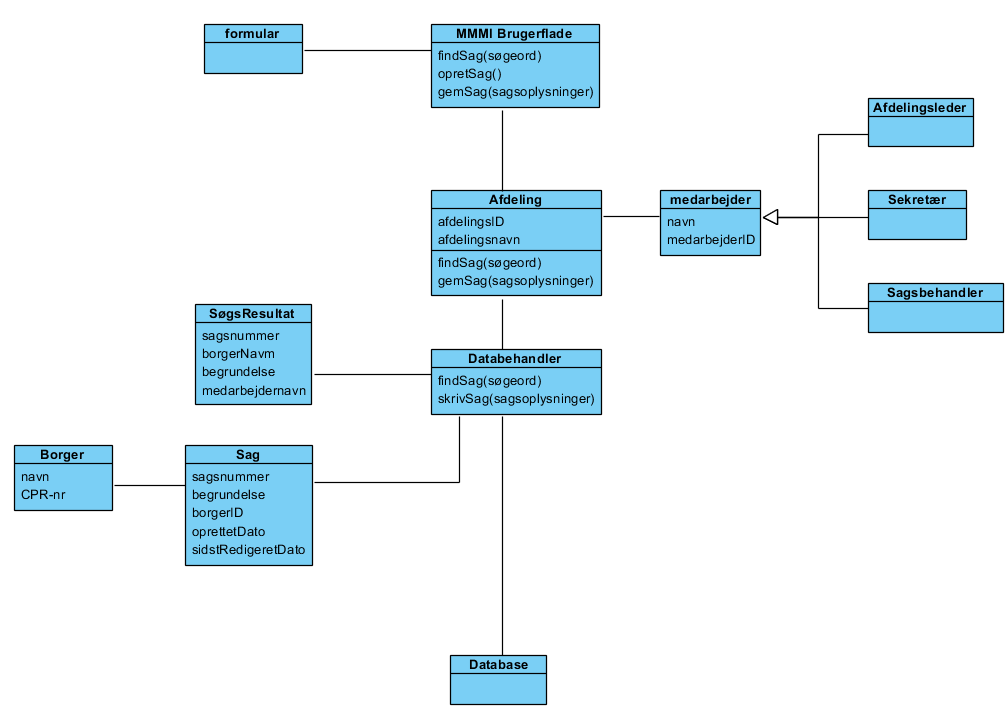
\includegraphics[scale = 0.7]{./PNG/analyse/analyseklassediagramOpdateret.PNG} 
  \caption{Opdateret analyseklassediagram}
  \label{fig:2analyseklasse}
\end{figure}
Da der har været fokus på at få integreret en database og en funktionel grafisk brugergrænseflade i 2. iteration, består de primære ændringer i den statiske analyse, af arbejdet med at revidere klassediagrammet, med henblik på at tilføje persistens og præsentation. Der er bl.a. blevet ændret på hvordan de tre klasser der repræsenterer ansatte, og klassen der repræsenterer borgere, beskrives. \\
Der blev valgt at gå væk fra en overordnet abstrakt klasse (Se figur \ref{fig:AKlasse})kaldet ”Person”, som ”Borger”, ”Afdelingsleder”, ”Sekretær” og ”Sagsbehandler” klasserne arvede fra. En abstrakt klasse kaldet ”medarbejder” blev lavet, som ”Afdelingsleder”, ”Sekretær” og ”Sagsbehandler” arvede fra i stedet, og holdt ”Borger” som en separat klasse. Dette betød at ”Borger” fik navn og CPR-nr. som attributter, til forskel fra 1. iteration hvor den kun havde CPR-nr. og arvede navn fra ”Person”. Yderligere blev medarbejderID flyttet til superklassen, da alle arvende klasser skulle bruge den. \\
Det blev droppet at beholde ”Afgørelsesbrev” som klasse, da det gav mere mening at lægge den i præsentationslagets klasse ”Formular”, som også repræsenterer alle andre formularer der beskrives i VUM.\\
Klassen ”Sag” er blevet rykket ned til datalaget og kan tilgås gennem Databehandler klassen, som er den klasse der repræsenterer datalaget og skal varetage al kommunikation med databasen.\\
De vigtigste metoder og attributter, på diverse klasser, er blevet opdateret i forhold til den nye viden, der er blevet indsamlet gennem 2. iteration. Der er blevet lavet nye metoder er på klassen (Se figur \ref{fig:2analyseklasse})”MMMI Brugerflade”, som er ”findSag”, ”opretSag” og ”gemSag”. På klassen ”Afdeling” er metoderne ”findSag” og ”gemSag” blevet lavet og på klassen ”Databehandler” er ”findSag” og ”skrivSag” blevet lavet. De nye attributter som er tilføjet, er ”begrundelse”, ”borgerID”, ”oprettetDato” og ”sidstRedigeretDato” på ”Sag”. \\
Den nye klasse ”SøgsResultat”, bruges til at holde data samlet i forbindelse med en given søgning af en sag. De attributter som vises i klassen ”SøgsResultat”, repræsenterer en begrænset delmængde af hvad der gemmes når en sag oprettes, men det er nok til at en bruger vil være i stand til at identificere en given sag for at åbne den.\\
Klassen Database repræsenterer den postgresql database er blevet designet og implementeret i iteration 2 (Se interne bilag figur \ref{fig:database}).
\subsubsection{Den dynamisk side af analyse}
I anden iteration er der blevet udarbejdet operationssekvensdiagrammer i forhold til ”opretSag()”, ”opdaterSag()” og ”find()”. \\
Operationen ”opretSag()” (Se afsnit \ref{opret}) og ”opdaterSag()” (Se afsnit \ref{opdaterSag}) er operationer der stammer fra opretSag() (se figur \ref{fig:opretSag}) fra første iteration. \\
Operationen find() er udviklet ud på baggrund af operationen ”findSag()” (se figur \ref{fig:findSag}) fra første iteration.\\ \\
\textbf{opretSag():} \label{opret} \\ 
Operationen ”opretSag()” er den funktion der opretter en sag i systemet. Der gjort overvejelser om at håndtere opdaterSag() i samme funktion som ”opretSag()”, men det ville ikke give mening. Derfor er de adskilt i to operationer. \\
I figur \ref{fig:2opret} begynder funktionen ved at en sagsbehandler eller sekretær vælger ”opretSag()”. Brugergrænsefladen returner en sagsåbningsformular, som skal udfyldes. Når sagsbehandleren har indtastet sagsoplysningerne vælger sagsbehandler at gemme sagen. Operationen ”gemSag()” sender besked til Afdeling som derefter benytter operationen ”skrivSag()” til Databehandleren og til sidst sender Databehandleren informationen videre til databasen. Databasen returner en bekræftelse til Databehandleren som returner den gennem Afdeling og brugerfladen som til sidst fortæller aktøren at sagen blev oprettet.
\begin{figure}[htb!]
  \includegraphics[scale = 0.5]{./PNG/analyse/opretsag2.PNG} 
  \caption{Opdateret sekvensdiagram for opret sag. For fuld størrelse se interne bilag \ref{sec:diverse} figur \ref{fig:2fopretsag}}
  \label{fig:2opret}
\end{figure}
Ved at anvende ”opretSag()” operationen har en sagsbehandler eller sekretær mulighed for at vælge en formular og ud fra den gemme og dermed oprette en ny sag. Oprettelsen sker når borgeren henvender sig og dermed kan sekretæren eller sagsbehandleren oprette en sag på den pågældende borger. For at kunne håndtere om en borger allerede har en sag eller om der findes oplysninger om borgen, benyttes ”find()” operation, som kan læses i afsnit \ref{find} \\
\begin{figure}[htb!]
  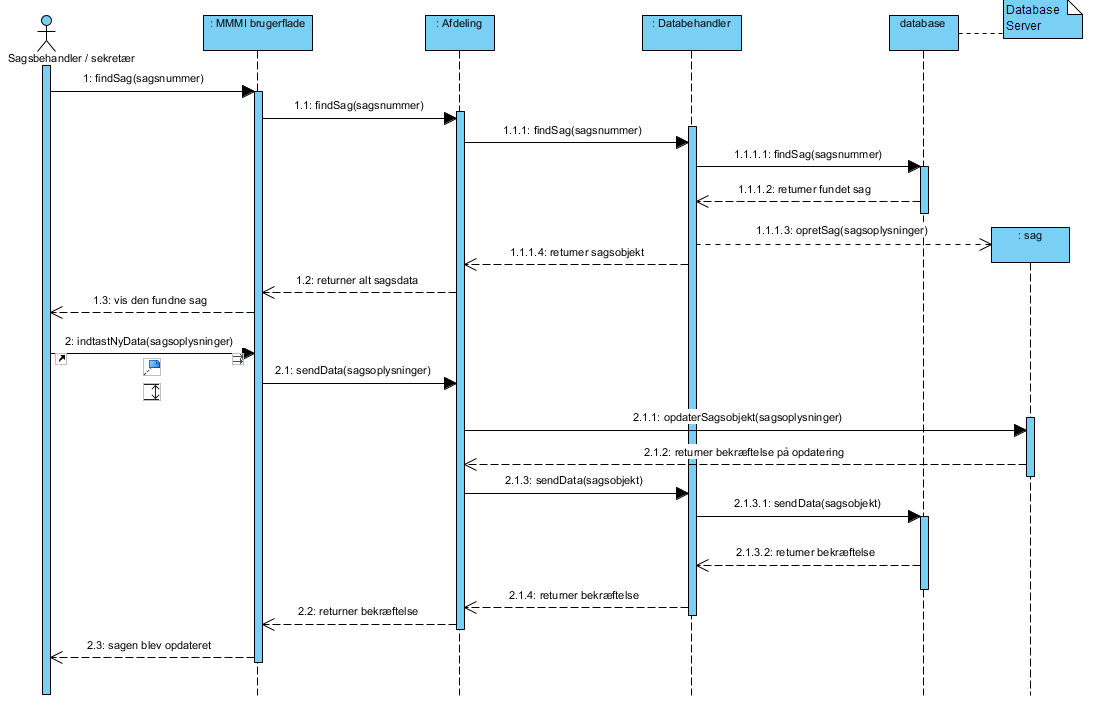
\includegraphics[scale = 0.62]{./PNG/analyse/opdaterSag.PNG} 
  \caption{Opdateret sekvensdiagram for opdater sag.}
  \label{fig:2opdater}
\end{figure} \\ \\
\textbf{opdaterSag():} \label{opdaterSag}\\
Operationen ”opdaterSag()” i kombination med ”find()” operationen gør det muligt for en aktør at kunne finde en specifik sag og dermed åbne den og opdatere den.  \\
I figur \ref{fig:2opdater} ses det at en sagsbehandler eller sekretæren vælger at fremsøge en sag. ”findSag()” beskeden bliver sendt igennem afdelingen og databehandleren. Databehandleren sørger for at sende beskeden til databasen og fremskaffe den søgte sag. Denne returneres til databehandleren og der bliver oprettet et sagsobjekt. Dette sagsobjekt returneres til afdelingen og herefter til brugerfladen som til sidst bliver præsenterer det til brugeren. Når brugeren har indtastet ny data sendes det til afdelingen via operationen ”sendData()”. Afdelingen sørger for at opdatere sagsobjektet gennem beskeden ”opdaterSagsobjekt()” hvor sag returner bekræftelse på opdaterede oplysninger er gemt. Det opdaterede sagsobjekt sendes til Databehandleren gennem beskeden ”sendData()” som derefter sender besked til databasen om at gemme de nye oplysninger. Der returneres en bekræftelse gennem databehandleren, afdelingen og brugerfladen som så bekræfter overfor aktøren at sagen blev opdateret.  \\ \\
\textbf{find():} \label{find}\\
Tanken med ”findSag()” i første iteration afsnit \ref{af:findSag} har været at kunne fremsøge en sag.\\
\begin{figure}[htb!]
  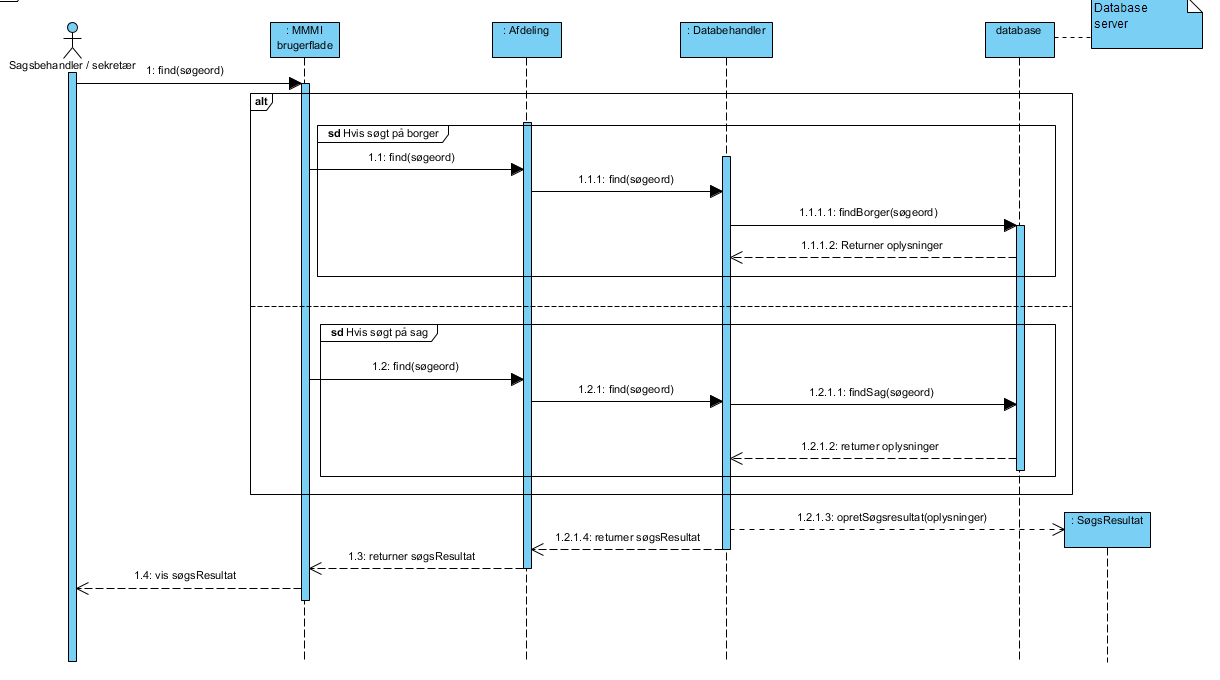
\includegraphics[scale = 0.56]{./PNG/analyse/find.PNG} 
  \caption{Opdateret sekvensdiagram for find sag.}
  \label{fig:2find}
\end{figure} 
\\ \\ \\
I figur \ref{fig:2find} vælger en sagsbehandler eller sekretær at finde en sag baseret på indtastet søgekriterier. Præsentationslaget sender ”find()” søgeord videre til Afdelingen, som sender det videre til Data- behandleren. Der søges i databasen, hvor det resultat der kommer fra database sendes til Data- behandleren der så, opretter et SøgsResultat objekt, som Databehandleren sender tilbage. Afdelingen sørger for at sende data til brugerfladen som til sidst viser resultatet af søgningen til aktøren. \\ 